\documentclass{article}
\usepackage[utf8]{inputenc}
\usepackage[spanish]{babel}
\usepackage{listings}
\usepackage{graphicx}
\usepackage{geometry}
\graphicspath{ {images/} }
\usepackage{cite}

\geometry{
textheight=23cm}
\begin{document}

\begin{titlepage}
    \begin{center}
        \vspace*{1cm}
            
        \Huge
        \textbf{INFORMA2 S.A.S}
            
        \vspace{0.5cm}
        \LARGE
        Parcial 2: Implementación
            
        \vspace{5cm}
            
        \textbf{Juan Pablo Cruz Gómez}
        
        \vspace{0.5cm}
        
        \textbf{Erika Dayana León Quiroga}
            
        \vfill
            
        \vspace{0.8cm}
            
        \Large
        Despartamento de Ingeniería Electrónica y Telecomunicaciones\\
        Universidad de Antioquia\\
        Medellín\\
        Septiembre de 2021
            
    \end{center}
\end{titlepage}

\tableofcontents
\newpage
\section{Sección introductoria}\label{intro}
En este informe se mostrará y explicará la implementación del problema presentado en el Parcial 2 de la materia Informática II, también se mostrarán las clases implementadas, los módulos del código implementado, la estructura del circuito montado en Tinkercad para la demostración del programa y los problemas que se presentaron durante el desarrollo de la implementación del problema.

\section{Clases implementadas} \label{clases}
En esta sección se presentarán las clases que se utilizarán para la solución del problema planteado.

\subsection{Clase QImage.}
Esta clase es proporcionada por Qt, sirve para el manejo de datos de imágenes, especialmente para el acceso y manipulación de pixeles. En este caso se utilizan los métodos que nos permiten conocer el número de pixeles a lo ancho y a lo largo de la imagen (.width, .height), para de esta forma obtener su tamaño. También se utiliza el método .pixelColor el cual retorna el color del pixel en unas coordenadas determinadas, en el caso de este problema se utiliza el .pixelColor dentro de un doble ciclo for que nos proporciona cada una de las coordenadas de la imagen, y de esta forma obtenemos la intensidad de color en cada uno de los pixeles de la imagen.



\section{Módulos del código implementado} \label{Modulos}
\begin{enumerate}
\item En esta parte del código se leen cada uno de los pixeles de la imagen para guardar su intensidad de color rojo, verde y azul, se hace uso de una matriz tridimensional llamada MatrizRGB para este propósito.

\begin{figure}[h]
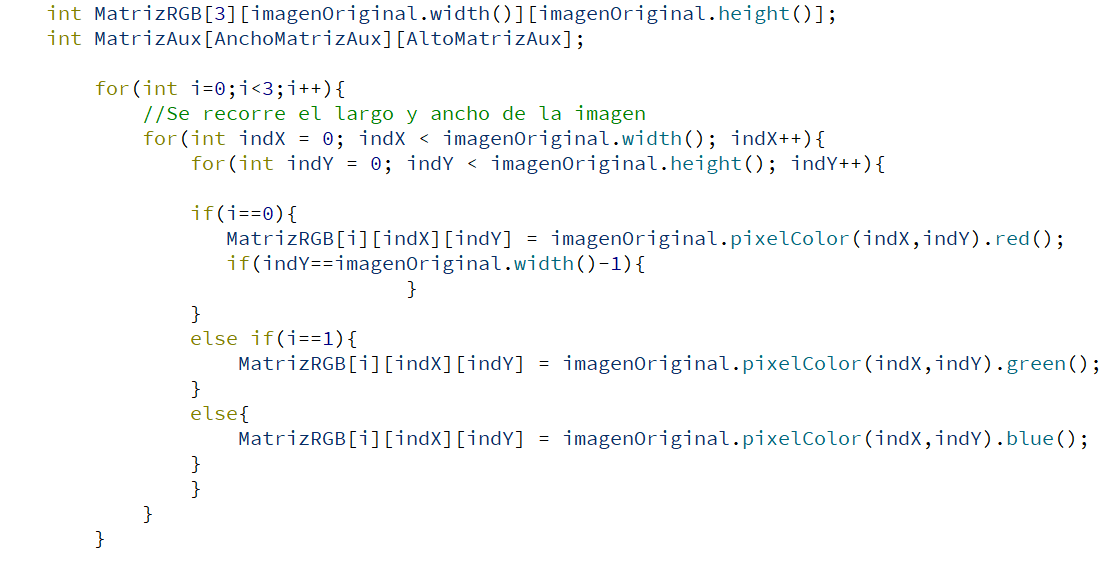
\includegraphics[width=15cm]{moduloMatrizRGB.png}
\centering
\caption{Matriz RGB}
\label{fig:matrizRGB}
\end{figure}

\item
\begin{figure}[h]
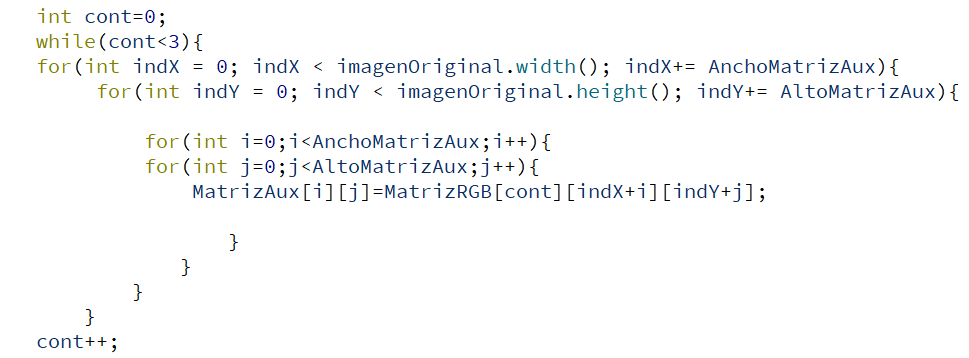
\includegraphics[width=15cm]{matrizaux.png}
\centering
\caption{Matriz RGB}
\label{fig:matrizaux}
\end{figure}


\end{enumerate}

\section{Estructura del circuito} \label{circuito}

\begin{figure}[h]
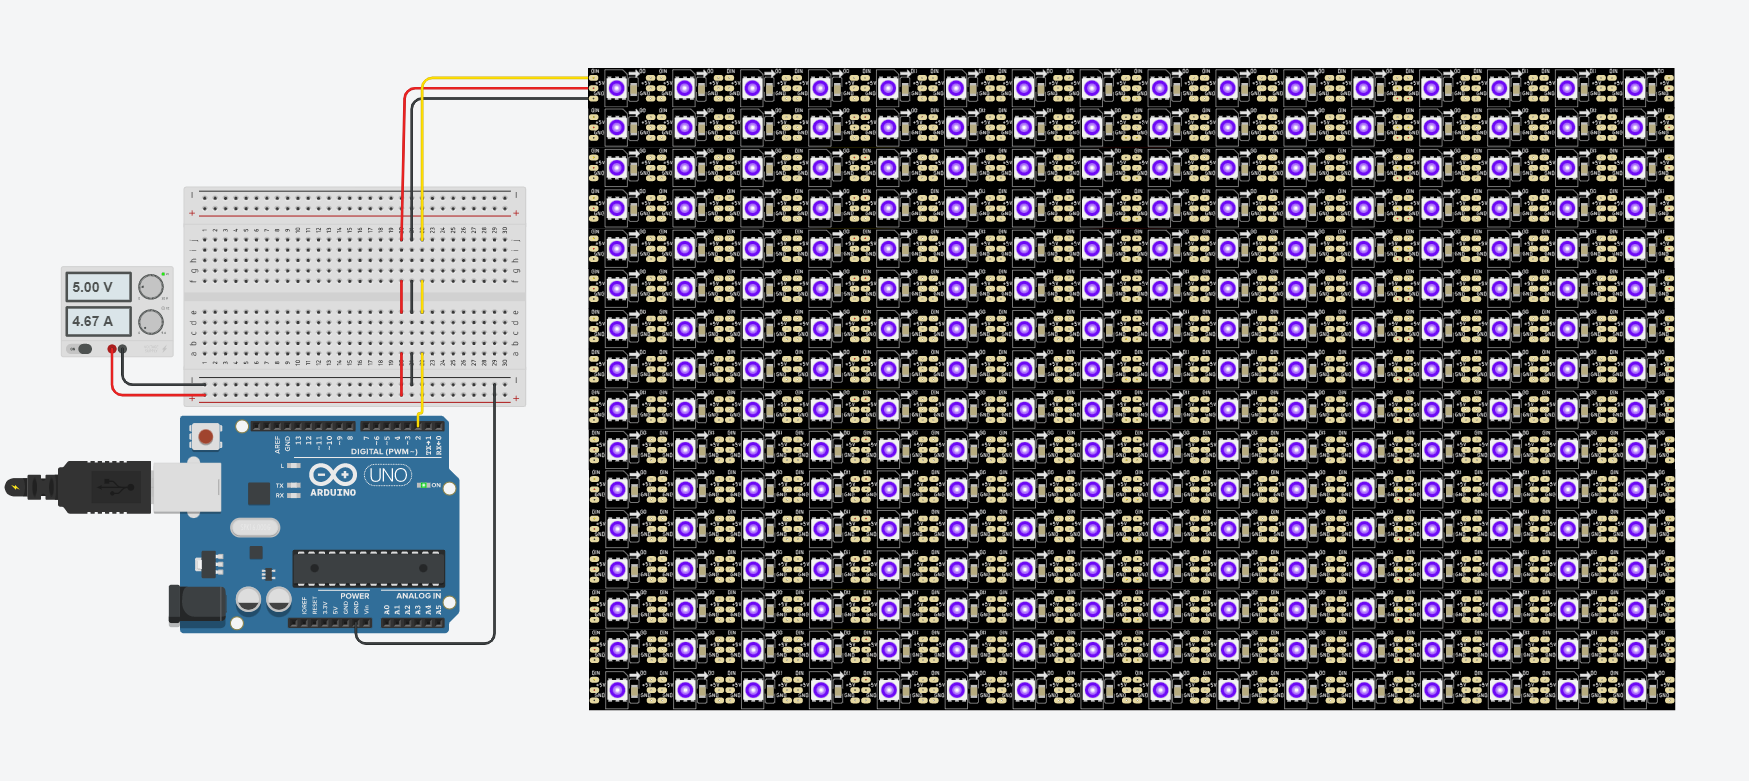
\includegraphics[width=15cm]{LEDs16x16.png}
\centering
\caption{Montaje de la matriz de LEDs de 16x16}
\label{fig:punto1}
\end{figure}


\section{Problemas presentados} \label{problemas}


\end{document}
